\chapter{Criptografia Moderna}
\label{cha:criptografia-moderna}

No final dos anos 40, com o desenvolvimento dos primeiros computadores e a experiência da quebra das cifras mecanicamente produzidas por poderosas máquinas desenvolvidas pelo esforço de guerra do nazismo, alguns cientistas se voltaram para um problema central no campo da criptografia: o que torna um sistema de criptografia seguro?

As cifras que vimos até agora são conhecidas como {\em cifras clássicas} exatamente porque elas precedem esse debate moderno, e não é à toa que foram todas derrotadas cedo ou tarde.
Informalmente, poderíamos dizer que o problema dos esquemas clássicos de criptografia é que eles mantêm muita informação sobre a mensagem original, como a frequência das letras, dos dígrafos, letras duplas, entre outros.
Esses padrões permitem que criptanalistas descubram o texto original sem conhecer a chave.

Não é uma coincidência, portanto, que a primeira tentativa de formalizar o conceito de segurança tenha sido proposta por Claude Shannon, o fundador da teoria da informação.
Shannon introduziu conceitos fundamentais que ajudaram a definir o que faz um sistema de criptografia ser verdadeiramente seguro.
Sua abordagem foi a base para o desenvolvimento de métodos mais robustos e seguros de criptografia.

\section{Sigilo Perfeito}
\label{sec:sigilo-perfeito}

Shannon definiu o que hoje chamamos de sigilo perfeito.
Um sistema de criptografia garante o {\em sigilo perfeito} se a probabilidade da mensagem original for independente da probabilidade da cifra.

Vamos relembrar o que são eventos independentes.
A probabilidade da mensagem original ser $m$ dado que a cifra é $c$ deve ser igual à probabilidade da mensagem ser $m$ independentemente da cifra.
Em termos matemáticos, isso significa que:

\begin{displaymath}
  Pr[M = m | C = c] = Pr[M = m]
\end{displaymath}

É nesse sentido preciso que dizemos que a cifra $c$ não guarda nenhuma informação sobre a mensagem $m$.
Quando essa condição é satisfeita, mesmo que um interceptador obtenha a cifra $c$, ele não obtém nenhuma pista sobre qual era a mensagem $m$.
Todas as mensagens possíveis são igualmente prováveis, tornando a criptoanálise impossível.
Ou seja, podemos dizer que um sistema de criptografia garante o sigilo perfeito se as cifras produzidas por ele não guardam informação da mensagem original.

De forma equivalente, um sistema de criptografia garante o sigilo perfeito se uma cifra $c$ qualquer pode ter sido produzida com igual probabilidade por qualquer mensagem $m$.
Dada uma cifra $c$ e duas mensagens $m_1$ e $m_2$ quaisquer, temos que:

\begin{displaymath}
  Pr[C = c | M = m_0] = Pr[C = c | M = m_1]
\end{displaymath}


A cifra de substituição não garante o sigilo perfeito. Vamos ver um exemplo simples que mostra isso.

Suponha que nossa cifra é {\tt OVO}.
Vamos calcular a probabilidade de diferentes mensagens originais terem gerado essa cifra.

Se a mensagem original for {\tt ana}, e usamos uma cifra de substituição específica que mapeia {\tt a} para {\tt O} e {\tt n} para {\tt V}, a mensagem cifrada resultante seria {\tt OVO}.
Se a chave, que nesse caso é uma permutação, foi escolhida de forma aleatória, temos 1 chance em 23 que a letra {\tt a} da mensagem original tenha sido substituída por {\tt O} na cifra.
A chance de {\tt n} ser substituído por {\tt V} é então 1 em 22, porque {\tt n} não pode ser substituído por {\tt O} que já foi escolhido.
Portanto, a probabilidade da mensagem original {\tt ana} gerar a cifra {\tt OVO} é $\frac{1}{22.23} = \frac{1}{650}$.

Agora, considere outra mensagem possível, como {\tt eva}.
Se a letra {\tt e} fosse substituída por {\tt O}, isso não seria possível porque {\tt a} também precisaria ser substituída por {\tt O}.
No entanto, na cifra de substituição, uma letra só pode ser mapeada para uma outra única letra, não duas vezes para a mesma letra.
Portanto, a probabilidade de a mensagem original ser {\tt eva} e gerar a cifra {\tt OVO} é 0.

Esse exemplo simples demonstra que as mensagens originais {\tt ana} e {\tt eva} têm probabilidades diferentes de gerar a cifra {\tt OVO}.
Em outras palavras, a cifra de substituição não garante o sigilo perfeito, pois a probabilidade da cifra ser gerada não é independente da mensagem original.
Portanto, algumas mensagens têm uma probabilidade maior de gerar uma cifra específica do que outras, o que pode fornecer pistas para a criptoanálise.

Outra forma de definir o sigilo perfeito é por meio de um jogo entre o sistema de criptografia $\Pi = \langle Gen, E, d \rangle$ e um adversário $\mathcal{A}$ que quer decifrá-lo.
O jogo funciona da seguinte maneira:

\begin{enumerate}
\item O adversário ($\mathcal{A}$) escolhe duas mensagens quaisquer $m_0$ e $m_1$.
  A única restrição é que elas devem ter o mesmo tamanho.
  O adversário então envia essas duas mensagens para o sistema $\Pi$.
\item O sistema então sorteia uma chave $k$ usando o algoritmo $Gen$ e escolhe aleatoriamente uma das duas mensagens.
\item O sistema criptografa a mensagem escolhida com a chave gerada  ($E(k,m) = c$) e devolve a cifra resultante $c$ para o adversário.
\item O adversário pode utilizar todos os meios ao seu dispor para descobrir qual das duas mensagens foi criptografada.
\end{enumerate}

Um sistema de criptografia garante o sigilo perfeito se, ao final do jogo, o adversário não tiver nenhuma vantagem em descobrir qual mensagem foi criptografada.

\begin{center}
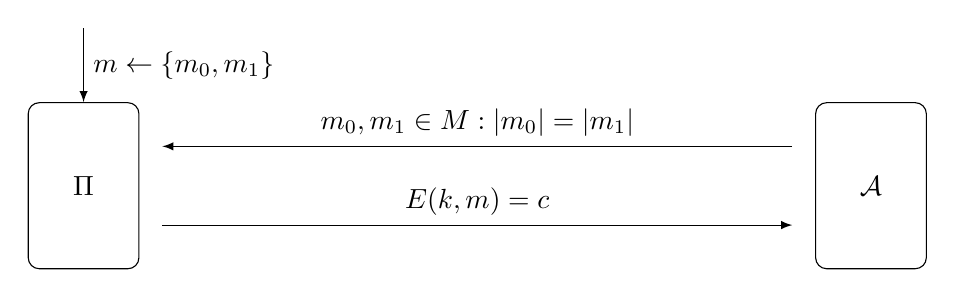
\begin{tikzpicture}[node distance=2cm,auto,>=latex]
\tikzset{
  player/.style={draw,shape=rectangle,rounded corners,minimum width=4em,minimum height=6em}
}
\node[player] (system) {$\Pi$};
\node[player] (adversary) at (10,0) {$\mathcal{A}$};
\draw[->] (9,.5) -> node[above]{$m_0, m_1 \in M : |m_0| = |m_1|$} (1,.5);
\draw[->] (1,-.5) -> node[above]{$E(k,m) = c$} (9,-.5);
\draw[->] (0,2) -> node{$m \leftarrow \{m_0,m_1\}$} (system);
%\draw[->] (adversary) -> node{$b' \in \{0,1\}$} (10,-2);
\end{tikzpicture}
\end{center}

Note que mesmo sem nenhuma informação, o adversário pode acertar qual das duas mensagens foi cifrada com $50\%$ de probabilidade, simplesmente chutando uma das duas.
O sistema $\Pi$ garante sigilo perfeito se isso for o melhor que o adversário pode fazer.
Ou seja, se a probabilidade de que ele vença o jogo for exatamente $\frac{1}{2}$

Apresentar esse conceito como um jogo enfatiza que a única informação que o adversário possui é a cifra que foi gerada pelo sistema.
Para que o sistema garanta sigilo perfeito, o conhecimento sobre a cifra não deve dar nenhuma vantagem ao adversário para que ele consiga distinguir qual das mensagens foi criptografada.

\section{One Time Pad}
\label{sec:otp}

Temos agora uma definição formal de segurança.
Vimos que a cifra de substituição não satisfaz essa definição, mas na verdade nenhuma das cifras clássicas a satisfaz.
As cifras clássicas, como a cifra de César, a cifra de substituição e a cifra de Vigenère, possuem vulnerabilidades inerentes que permitem que adversários determinem informações sobre a mensagem original a partir da cifra.

Não seria desejável que essas cifras satisfizessem a definição de sigilo perfeito, pois vimos no capítulo anterior que nenhuma das cifras clássicas é segura.
Todas elas podem ser derrotadas se o adversário tiver acesso a uma cifra de tamanho suficientemente grande.
Por exemplo, a análise de frequência pode ser usada para quebrar cifras de substituição, enquanto técnicas como o método de Kasiski podem ser aplicadas para quebrar a cifra de Vigenère.

A definição de sigilo perfeito nos fornece um padrão muito elevado de segurança, onde a cifra não revela absolutamente nenhuma informação sobre a mensagem original.
Este é um objetivo ideal para sistemas de criptografia, pois garantiria que mesmo um adversário com poder computacional ilimitado não pudesse descobrir a mensagem original a partir da cifra.

Ficamos então com o desafio de encontrar algum sistema que satisfaça essa definição, caso tal sistema exista.
Esta busca nos leva a explorar técnicas e métodos mais avançados de criptografia.
Claude Shannon, em seus estudos, encontrou um sistema assim chamado de {\em One-Time Pad} (OTP).

No que segue, apresentaremos um sistema chamado One Time Pad, também conhecido como {\em cifra de Vernam}, e mostraremos que ele garante o sigilo perfeito.
A partir deste ponto, conforme começarmos a investigar sistemas a serem implementados computacionalmente, consideraremos que o espaço das mensagens (assim como o espaço das cifras) será representado não mais como sequências de letras, mas como sequências de bits.

No caso específico do OTP, assumiremos que as mensagens e as cifras possuem um tamanho fixo.
Mais importante é o fato de que o universo das chaves é também um conjunto de sequências de bits {\em do mesmo tamanho}.
Em outras palavras, tanto as mensagens quanto as chaves e as cifras serão representadas por sequências de $n$ bits.

O OTP é um sistema de criptografia:
\begin{itemize}
\item $Gen$ sorteia uma chave $k$ de $n$ bits.
\item Para criptografar uma mensagem $m$, que também é uma sequência de $n$ bits, realizamos uma operação bit a bit (bitwise) chamada de XOR (ou exclusivo) entre a mensagem $m$ e a chave $k$:
  \begin{displaymath}
    c = k \xor m
  \end{displaymath}
\item Para descriptografar a cifra $c$, aplicamos novamente a operação XOR entre a cifra $c$ e a mesma chave $k$:
  \begin{displaymath}
    k \xor c
  \end{displaymath}
\end{itemize}

A operação XOR entre dois bits é definida como:

\begin{eqnarray*}
  0 \xor 0 & = & 0\\
  1 \xor 0 & = & 1\\
  0 \xor 1 & = & 1\\
  1 \xor 1 & = & 0
\end{eqnarray*}

A operação XOR entre sequências de bits possui algumas propriedades que serão úteis.
Deixamos como exercício mostrar essas quatro propriedades da operação:

\begin{itemize}
\item (idempotência) $m \xor m = 0$
\item (identidade) $m \xor 0 = m$
\item (comutatividade) $m \xor n = n \xor m$
\item (associatividade) $(m_1 \xor m_2) \xor m_3 = m_1 \xor (m_2 \xor m_3)$
\end{itemize}

Essas propriedades são suficientes para mostrar que o sistema é correto.
Ou seja, se criptografamos uma mensagem ($m$) produzindo uma cifra ($E(k,m) = c$) e depois descriptografamos essa cifra ($c$) com a mesma chave $D(k,c)$ recuperamos a mensagem original.

\begin{itemize}
\item $E(k,m) = k \xor m = c$
\item $D(k,c) = k \xor c = k \xor (k \xor m)$
\item $D(k,c) = (k \xor k) \xor m$ por associatividade
\item $D(k,c) = 0 \xor m$ por idempotência
\item $D(k,c) = m$ por identidade
\end{itemize}

\begin{example}
  Considere uma mensagem $m = 101010$ e uma chave $k = 010001$.
Usando o sistema One Time Pad a cifra produzida é a seguite:

\begin{displaymath}
  \begin{array}{ccccc}
    m & \xor & k & = & c \\
    101010 & \xor & 010001 & = & 111011
  \end{array}
\end{displaymath}
\end{example}




Como antecipado, é possível, e relativamente simples provar que o OTP possui sigilo perfeito.

\begin{theorem}
  O sistema de criptografia {\em One Time Pad} possui sigilo perfeito.
\end{theorem}

Para provar o teorema note dada uma cifra $c$ que esiste uma única chave $k$ tal que $E(k,m = c)$, a saber $k = c \xor m$:

  \begin{eqnarray*}
    E(k, m) & = & k \xor m \\
            & = & (c \xor m) \xor m\\
            & = & c \xor (m \xor m)\\
            & = & c \xor 0\\
            & = & c
  \end{eqnarray*}

Agora, a probabilidade de escolher essa chave específica entre todas as possíveis chaves (sequências de bits de comprimento $n$) é $\frac{1}{2^n}$.

Isso significa que a probabilidade de obter a cifra $c$ a partir de qualquer mensagem $m$ é a mesma, independente de qual mensagem foi escolhida originalmente.
Essa probabilidade é sempre $\frac{1}{2^n}$.

Portanto, a cifra $c$ é igualmente provável para qualquer mensagem $m$.
Em outras palavras, o conhecimento da cifra $c$ não fornece ao adversário nenhuma informação adicional sobre qual mensagem foi originalmente enviada, garantindo assim o sigilo perfeito.

O One Time Pad (OTP) possui duas severas limitações que afetam sua aplicação prática.

A primeira limitação é indicada pelo próprio nome do sistema.
O OTP pressupõe que a chave de criptografia $k$ seja usada exatamente uma vez, ou seja, ``one time''.
Isso significa que cada chave deve ser única e exclusiva para uma única mensagem.
Se a mesma chave $k$ for reutilizada para criptografar duas mensagens distintas $m_1$ e $m_2$, o sistema se torna completamente inseguro.

Para ilustrar essa limitação considere que duas cifras $c_0$ e $c_1$ foram produzidas usando a mesma chave $k$.
Assim temos que $c_0 = k \xor m_0$ e $c_1 = k \xor m_1$.
Note o que acontece quando aplicamos o ou exclusivo entre as duas cifras eliminamos a chave:

\begin{eqnarray*}
  c_0 \xor c_1 & = & (k \xor m_0) \xor (k \xor m_1)\\
              & = & (k \xor k) \xor (m_0 \xor m_1)\\
              & = & m_0 \xor m_1
\end{eqnarray*}

Isso significa que o adversário pode obter a operação XOR das duas mensagens originais, mesmo sem conhecer a chave $k$.

Com essa informação, o adversário pode realizar uma análise de frequência ou outras técnicas de criptoanálise para tentar deduzir as mensagens originais, especialmente se as mensagens tiverem algum padrão ou conteúdo previsível.
Esse tipo de ataque é conhecido como {\em ataque de reutilização de chave}, e mostra que a segurança do OTP depende criticamente do uso único de cada chave.

Portanto, a reutilização de uma chave no OTP compromete a segurança do sistema, transformando-o de um sistema teoricamente perfeito em um sistema vulnerável e facilmente quebrável.

A segunda e mais crítica limitação do OTP é o tamanho de sua chave.
A suposição que fizemos é que o tamanho da chave deve ser tão grande quanto a mensagem a ser cifrada.
Há uma série de problemas práticos com isso.
Computacionalmente, não é possível gerar chaves aleatórias muito grandes, o que limita o tamanho das mensagens que podemos cifrar.

Além disso, assumimos que as chaves são compartilhadas entre as partes.
Deixamos os detalhes sobre a distribuição de chaves para o Capítulo \ref{cha:distribuicao-chaves}, mas por ora podemos adiantar que se nossa chave é tão grande quanto a mensagem, por que não enviamos a mensagem pelo mesmo canal que enviaríamos a chave?
Esse é um ponto crítico, pois, se conseguimos enviar a chave de forma segura, poderíamos, em teoria, enviar a mensagem diretamente pelo mesmo canal, tornando o uso da chave redundante.

Enfim, um sistema cuja chave seja tão grande quanto a mensagem é de muito pouca utilidade prática.
A dificuldade de gerar, distribuir e gerenciar chaves de tamanho adequado para cada mensagem limita significativamente a aplicabilidade do OTP em contextos reais.

Encerramos este capítulo mostrando que esta segunda limitação do OTP infelizmente não é uma peculiaridade do sistema.
Na verdade todo sistema que possua sigilo perfeito está fadado a ter chaves tão grandes ou maiores do que a mensagem.
Esse resultado negativo foi proposto e demonstrado pelo próprio Shannon ainda nos anos 40.


\begin{theorem}[Shannon]
Se um sistema que garante o sigilo perfeito, então seu universo de chaves deve ser pelo menos tão grande quanto seu universo de mensagens, ou seja, o tamanho da chave deve ser maior ou igual ao tamanho da mensagem.
\end{theorem}

Consideremos $M(c)$ como o conjunto de todas as mensagens que podem produzir a cifra $c$.

O tamanho de $M(c)$ deve ser menor ou igual ao número de chaves disponíveis.
Isso é porque, se uma mesma chave pudesse produzir $c$ a partir de mensagens diferentes, a descriptografia não funcionaria corretamente, pois não poderíamos determinar qual mensagem foi originalmente cifrada.

Agora, imagine que o número de chaves seja estritamente menor do que o número de mensagens.
Nesse caso, haveria pelo menos uma mensagem $m$ que não estaria em $M(c)$, ou seja, uma mensagem que não pode gerar a cifra $c$.

Isso significa que a probabilidade das mensagens não seria independente da probabilidade das cifras. Para essa mensagem $m$, teríamos:
\begin{itemize}
\item A probabilidade de escolher $m$ não seria zero: $Pr[M = m] \neq 0$
\item A probabilidade de $m$ produzir $c$ seria zero: $Pr[M = m | C = c] = 0$
\end{itemize}

Ou seja, se houver mais mensagens do que chaves, haveria mensagens que não poderiam produzir certas cifras, tornando a probabilidade das mensagens dependente das cifras.
Portanto, para garantir o sigilo perfeito, o número de chaves deve ser pelo menos igual ao número de mensagens.

A definição de segurança proposta por Claude Shannon foi a primeira tentativa séria de formalizar a segurança dos sistemas de criptografia.
No entanto, o próprio Shannon demonstrou as limitações dessa definição.
Nos próximos capítulos, apresentaremos definições de segurança mais fracas, porém mais práticas e úteis para nossos propósitos.

Shannon definiu que um sistema de criptografia garante o sigilo perfeito se a cifra não guarda nenhuma informação sobre a mensagem que a produziu.
Em outras palavras, qualquer possível mensagem é igualmente provável, independentemente da cifra interceptada pelo adversário.
Essa definição estabelece um padrão de segurança extremamente elevado e teórico.

Como acabamos de ver, apesar da robustez teórica, a definição de sigilo perfeito tem uma limitação prática significativa:
ela exige que o universo de chaves seja pelo menos tão grande quanto o universo das mensagens.
Isso significa que, para cada mensagem possível, deve existir uma chave única que possa ser utilizada para cifrá-la, resultando em um número enorme de chaves que precisam ser geradas, distribuídas e armazenadas de maneira segura.

Apesar do fracasso desta primeira tentativa de formalizar o conceito de segurança, não abandonaremos a ideia geral.
A abordagem da {\em criptografia moderna} \cite{Goldwasser84}, que utilizaremos nesta apostila, segue três princípios básicos:
\begin{enumerate}
\item {\em definições formais:}
  As noções de segurança utilizadas serão apresentadas de maneira formal por meio de definições claras.
  Essas definições nos ajudam a comparar diferentes sistemas de criptografia e avaliar sua segurança com base em critérios previamente estabelecidos.
\item {\em suposições explícitas:}
  Muitas vezes, precisamos fazer suposições sobre os sistemas de criptografia que não podemos provar.
  No entanto, é crucial que essas suposições sejam explicitadas de maneira clara e formal.
  Mesmo sem provas definitivas, podemos validar essas suposições empiricamente.
  Grande parte do trabalho na criptografia moderna envolve testar essas suposições e buscar as mais simples e básicas.
\item {\em demonstrações formais:}
  Quando conseguimos formalizar nossas suposições e definir a segurança desejada, podemos eventualmente provar que um sistema que atende a essas suposições garante uma certa noção de segurança.
  Esse tipo de demonstração reduz o problema da segurança às suposições do sistema, que devem ser mais simples e mais fáceis de validar empiricamente.
  Essa abordagem permite substituir um sistema se suas suposições forem refutadas, antes que ele seja quebrado.
\end{enumerate}

As definições de segurança em criptografia geralmente possuem dois componentes: uma garantia de segurança e um modelo de ameaças.
\begin{itemize}
\item {\em Garantia de Segurança:} Especifica o que pode ser considerado um ataque bem-sucedido.
\item {\em Modelo de Ameaças:} Define o que o adversário pode ou não pode fazer.
\end{itemize}

Por exemplo, na definição de sigilo perfeito, a garantia de segurança é que nenhuma informação sobre a mensagem esteja contida na cifra.
Isso significa que a probabilidade de ocorrência da cifra deve ser independente da probabilidade de ocorrência da mensagem.
O modelo de ameaças assume que o adversário tem acesso apenas ao texto cifrado e nada mais.
Este modelo de ameaça é destacado na definição que demos, simulando um jogo entre o sistema de criptografia e um adversário.
No jogo, o adversário tenta adivinhar qual mensagem foi cifrada com base apenas na cifra recebida, sem qualquer informação adicional.

Os modelos de ameaças que estudaremos na apostila incluem:
\begin{itemize}
\item {\em ataque apenas ao texto cifrado (ciphertext-only):} 
  Este é o modelo assumido na definição de sigilo perfeito.
  Nele, supomos que o adversário tem acesso apenas a um texto cifrado de tamanho arbitrário.
\item {\em ataque com escolha de texto plano (ataque chosen-plaintext):}
  Neste modelo, além de assumir que o adversário tem acesso à cifra, supomos que ele é capaz de escolher algumas mensagens e ver como elas seriam cifradas pelo sistema.
  Isso dá ao adversário mais informações para tentar descobrir a chave de criptografia ou a mensagem original.
\item {\em ataque com escolha de texto cifrado (ataque chosen-ciphertext):}
  Neste modelo, assumimos que o adversário é capaz de escolher certas cifras e ver como elas seriam decifradas pelo sistema.
  Esse é um modelo de ameaça mais poderoso, pois permite ao adversário interagir com o sistema de criptografia de maneira mais direta e potencialmente descobrir vulnerabilidades.
\end{itemize}

Esses modelos de ameaças são progressivamente mais fortes, o que significa que cada um assume uma capacidade de ataque cada vez maior por parte do adversário.
É importante notar que nossos modelos de ataque não fazem suposições sobre a estratégia específica que o adversário pode usar.
Eles simplesmente definem o que o adversário é capaz de fazer em termos de acesso a informações e interações com o sistema de criptografia.
Isso nos permite avaliar a segurança de um sistema de maneira abrangente e rigorosa, sem depender de suposições específicas sobre o comportamento do adversário.

Nossa primeira tentativa de definir segurança encontrou uma limitação significativa expressa pelo teorema de Shannon.
Afirmamos no capítulo anterior que o sigilo perfeito pode ser definido por meio de um jogo, onde o sigilo perfeito é garantido se nenhum adversário for capaz de distinguir qual mensagem foi encriptada pelo sistema.
No entanto, essa definição rigorosa exige que o número de chaves seja pelo menos tão grande quanto o número de mensagens, o que não é prático.

Para contornar as limitações expressas pelo teorema de Shannon, enfraqueceremos essa definição de segurança de duas formas principais:
\begin{itemize}
\item {\em Adversário eficiente}:
  Assumiremos que o adversário deve ser eficiente, ou seja, ele deve usar sua estratégia em um tempo razoável.
  Na prática, isso significa que, embora um adversário possa eventualmente derrotar o sistema se lhe for dado tempo suficiente, essa possibilidade não viola nossa definição de segurança.
  A ideia é que, se o tempo necessário para o adversário quebrar o sistema é impraticavelmente longo, o sistema ainda pode ser considerado seguro.
  Portanto, a existência de um adversário que possa eventualmente derrotar o sistema, mas que necessite de um tempo excessivo para fazê-lo, não representa uma ameaça real na prática.
\item {\em Probabilidade pequena}:
  Permitiremos que o adversário possa eventualmente derrotar o sistema, mas apenas com uma probabilidade muito pequena.
  Em outras palavras, a cifra pode conter alguma informação sobre a mensagem original, desde que essa quantidade de informação seja insignificante.
  Isso significa que, embora não possamos garantir que a cifra seja completamente independente da mensagem, a informação que pode ser extraída deve ser tão mínima que não ofereça uma vantagem significativa ao adversário.
  Dessa forma, mesmo que exista uma pequena chance de o adversário descobrir algo sobre a mensagem, essa chance deve ser tão baixa que o sistema ainda é considerado seguro na prática.
\end{itemize}

Ao enfraquecer a definição de segurança dessa maneira, movemos de um ideal teórico inatingível para uma abordagem mais prática que ainda oferece altos níveis de segurança.
Este equilíbrio entre segurança teórica e viabilidade prática é fundamental na criptografia moderna, permitindo-nos desenvolver sistemas que são seguros o suficiente para resistir aos ataques dentro de limites de tempo e probabilidade razoáveis.

\section{Abordagem Assintótica}
\label{sec:abord-assint}

Em termos práticos, buscamos uma noção de segurança que imponha requisitos severos ao sucesso de um adversário.
Especificamente, queremos que um adversário precise rodar seu algoritmo em uma máquina extremamente poderosa por um intervalo de tempo muito grande para ter sucesso.
Alternativamente, esperamos que o adversário possa eventualmente derrotar o sistema em pouco tempo, mas com uma probabilidade extremamente baixa.

Em termos práticos, buscamos uma noção de segurança que imponha requisitos severos ao sucesso de um adversário.
Especificamente, queremos que um adversário precise rodar seu algoritmo em uma máquina extremamente poderosa por um intervalo de tempo muito grande para ter sucesso.
Alternativamente, esperamos que o adversário possa eventualmente derrotar o sistema em pouco tempo, mas com uma probabilidade extremamente baixa.

\begin{itemize}
\item {\em Máquina extremamente poderosa}:
  A definição de uma máquina poderosa varia com o tempo e o avanço da tecnologia.
  Uma máquina que hoje é considerada de ponta pode se tornar obsoleta em poucos anos.
  Portanto, qualquer definição baseada na capacidade atual das máquinas é inevitavelmente temporária.

\item {\em Intervalo bem grande de tempo}:
  Similarmente, o que consideramos um tempo razoavelmente longo para resistir a ataques também muda com o tempo.
  O que era considerado seguro há uma década pode não ser mais seguro hoje.
  Assim, definir um intervalo de tempo ``bem grande'' é complicado, pois deve se ajustar ao ritmo acelerado de avanços tecnológicos.

\item {\em Probabilidade muito baixa}:
  Determinar uma probabilidade de sucesso muito baixa para um ataque também é desafiador.
  Uma probabilidade aceitável hoje pode não ser aceitável amanhã à medida que as técnicas de ataque evoluem.
  Além disso, a definição de ``muito baixa'' deve ser precisa e quantificável, o que pode ser difícil de estabelecer de forma universal.
\end{itemize}

Em vez de estabelecer valores fixos para esses limites, adotamos uma abordagem assintótica, como fazemos ao analisar algoritmos ou avaliar a complexidade de um problema.
Vamos supor que, ao gerar a chave, o algoritmo $Gen$ recebe um parâmetro de segurança $n$ e estabelecemos nossos limites em função deste parâmetro.

Para os efeitos desta apostila, podemos assumir que o parâmetro está relacionado ao tamanho da chave a ser gerada e que é de conhecimento público.
O parâmetro de segurança permite que as partes ajustem seu sistema para o nível desejado de segurança.
Aumentar o parâmetro de segurança geralmente resulta em um aumento no tempo de processamento do sistema e no tamanho da chave.

A capacidade de ajustar o parâmetro de segurança tem vantagens práticas.
Ela permite que as partes defendam seus sistemas contra adversários com poder computacional mais forte à medida que o tempo passa e a tecnologia avança.
Isso significa que, à medida que novas técnicas de ataque e hardware mais poderoso são desenvolvidos, podemos simplesmente aumentar o parâmetro de segurança para manter o sistema protegido.

Com essa abordagem, podemos definir de maneira mais clara nossas garantias de segurança.
Vamos exigir que nenhum adversário rodando um {\em algoritmo polinomial} em relação ao tamanho do parâmetro de segurança $n$ seja capaz de distinguir as mensagens, exceto com uma probabilidade desprezivelmente maior que $\frac{1}{2}$.
Por ``desprezivelmente maior'', queremos dizer que esse valor cresce mais lentamente do que qualquer polinômio em relação a $n$.

Em termos práticos, isso significa que, conforme aumentamos o parâmetro de segurança, a probabilidade de um adversário bem-sucedido se torna insignificante.
Essa abordagem nos permite criar sistemas que são adaptáveis e capazes de fornecer altos níveis de segurança, mesmo diante de adversários com crescente poder computacional.


\section{Exercícios}
\label{sec:exercicios}

\begin{exercicio}
  Mostre que o $0$ é elementro neutro na operação $\xor$, ou seja, que para todo $x \in \{0,1\}^*$ temos que $x \xor 0 = 0 \xor x = x$.
\end{exercicio}

\begin{exercicio}
  Mostre que a operação $\xor$ é {\em associativa}, ou seja, que para todo $x,y,z \in \{0,1\}^*$ temos que $x \xor (y \xor z) = (x \xor y) \xor z$.
\end{exercicio}

\begin{exercicio}
  Mostre que a operação $\xor$ é {\em comutativa}, ou seja, que para todo $x,y \in \{0,1\}^*$ temos que $x \xor y = y \xor x$.
\end{exercicio}

\begin{exercicio}
  Mostre que para qualquer sequência de bits $x \in \{0,1\}^*$ temos que $x \xor x = 0$.
\end{exercicio}

\begin{exercicio}
  Sejam $\varepsilon_1$ e $\varepsilon_2$ duas funções desprezíveis.
  Mostre que $\varepsilon_1 + \varepsilon_2$ é desprezível.
\end{exercicio}

\begin{exercicio}
  Seja $\varepsilon$ uma função desprezível e $p$ um polinômio.
  Mostre que $p\varepsilon$ é desprezível.
\end{exercicio}

\begin{exercicio}
  Quais as vantagens da abordagem assintótica na definição da garantia de segurança?
\end{exercicio}

\begin{exercicio}
  Por que representamos o parâmetro de segurança em notação unária?
\end{exercicio}

\begin{exercicio}
  Considere um sistema $\Pi$ seguro contra ataques {\em ciphertext only} cujo parâmetro de segurança tem $128$ bits ($n = 128$) e um adversário polinomial que derrota o sistema com probabilidade $\frac{1}{2} + \frac{1}{2^{n/4}}$.
Com que probabilidade esse adversário derrotaria o sistema se dobrassemos $n$?
\end{exercicio}

\begin{exercicio}
  Considere um sistema $\Pi$ seguro contra ataques {\em ciphertext only} cujo parâmetro de segurança tem $128$ bits ($n = 128$) e um adversário que roda um algoritmo que derrota o sistema com probabilidade $1$ em $2^{n/8}$ passos.
  Quantos passos seriam necessários para esse algoritmo derrotar um sistema se dobrássemos $n$? E se quadrupicássemos $n$?
\end{exercicio}
